\section{RHUL Plasyss Depositer\label{sec:plassys}}
Machine in  separate room.  Used  for good deposition. For  flakes on
28th January we did 10nm of titanium and 80nm of aluminium.

\begin{framed}\noindent
  Orient the sample so that the axis of rotation goes parallel to the
  overlap you  want.  The  sample will rock  along this  axis, giving
  overlap  either side  of the  rotation axis.!   THIS IS  NEEDED FOR
  CORRECT ANGLE DEPOSITION

  Etching  may  be used  to  remove  oxidised  layers prior  to  main
  deposition for good ohmic contact.
\end{framed}

\subsection{Starting up}
\begin{itemize}
\item  \cmd{Turn on  \quote{mains} and  turn on  \quote{disconnector}
    dial \ira \quote{start}} (green button);
\item \cmd{\quote{Motor} \ira \quote{Home}} to remove warning;
\item   \cmd{Log   on   as    }\quote{engineer}   and   password   is
  \quote{password};
\item  \cmd{\quote{Ch Cryo}  \ira  \quote{Regen}} to  start the  cryo
  pump.   It purges  (fills up  with  nitrogen) and  pumps to  remove
  nitrogen and water vapour;
\end{itemize}
\subsection{Loading}
\begin{itemize}
\item  \texttt{Vent button  on the  \red{loadlock process  panel}} to
  vent the loadlock for 3 minutes.   When lid can be freely lifted up
  \red{and the  ATM LL  orange button above  the emergency  button is
    on}, you are ready.
\item \red{Wearing gloves},  remove the base from  Plassys by pushing
  and turning.
\item Attach the sample. Ensure that  it doesn't fall off when tipped
  upside down.
\item \red{In  gloves load the  base as  before.  Make sure  that the
    small circular  pin on  the base  is closest to  the door  of the
    lab.}
\item Close  the lid and  press the \texttt{pump  button}. \red{Press
    lid down for the first part of the pumping}.This will vent for 20
  or so minutes.  \red{Should be  around $10^{-7}$mBar when ready for
    use.}
\item   \cmd{To   rotate   the   stage,   go   to   \quote{planteray}
    menu. \red{The angle you enter will be halved by the program! }}
\item  \cmd{\red{Click   the  two-tirangle-facing-each-other}  symbol
    between the chambers on the diagram}  \ira it should go green, to
  indicate that the two chambers have been connected;
\end{itemize}

  \subsection{Creating a process for deposition}
  In order to make a custom process

  \begin{itemize}
  \item \texttt{Process editor \ira Add new process}.
  \item Always  have the  \texttt{Pump LL to  $5\times10^{-6}mBar$} +
    \texttt{Pump Ch to $5\times10^{-7}mBar$}
  \item \texttt{Insert row} to add a new step.
  \item Go to  folder on the left  hand side of the  screen, and drag
    the  required  new  processes  such as  \texttt{deposit  10nm  of
      aluminium}.
  \item \red{\texttt{Save as \ira new process}}.
  \end{itemize}

  \subsection{Running process}
  \begin{itemize}
  \item \texttt{Run process \ira select  sequence \ira file \ira open
      recipe}
  \item \texttt{Execute button} to run it.
  \item A series of heating up material, getting the right deposition
    rate, right  vacuum is performed.   There are frequent  checks yo
    which you must agree.
  \end{itemize}

  \subsection{Ending}
  \red{\begin{itemize}
    \item \texttt{Vent}  the loadlock and  wait for 3  minutes before
      removing with gloves;
    \item Make  sure you screw on  all the plates on  the base before
      replacing;
    \item {\Large Pump the system before leaving \ira ensure that the
        turbomolecular regime is reached;}
    \item \cmd{\quote{Loadlock} \ira \quote{Stop}} to stop pumping of
      chamber  once good  pressure is  reached in  order to  save the
      pump.
    \end{itemize}}

  \subsection{Static oxidation}
  For JJ  it is  required to  oxidise after the  first Al  layer, and
  after the whole process is  finished. The two options for oxidation
  are:
  \begin{itemize}
  \item \textbf{Static regime} is used, whereby $ \approx $ 0.3 or 10\,mbar
    (first layer  and second  layer oxidations)  of oxygen  is pumped
    into the chamber and we wait for 10minutres or so.
  \item \textbf{Dynamic regime} where a flow of $ \approx 40\mu$bar is shot
    at the sample.
  \end{itemize}

  \subsubsection{Static setup}
  For the static case, we need to adjust the needle valve (small turn
  dial in front  of red flow meter) so that  the required pressure is
  reached  after  30sec,  so   that  Plassys  doesn't  overshoot  the
  pressure;
  \begin{enumerate}
  \item \cmd{Pump the load lock to base pressure};
  \item \cmd{\red{Close the needle valve by turning it clockwise \ira
        unscrew it by 10\ideg or so}};
  \item \cmd{Click \quote{Oxidation \ira static} to engage the static
      mode};
  \item \cmd{Click  the two traingles  next to the  \quote{O2} symbol
      \red{between Ar and O2 t-junctions}} so that oxygen is let in;
  \item  \cmd{Time,  that  the   pressure  in  the  loadlock  reaches
      0.3\,mBar in around 30 seconds};
  \item  \cmd{\red{If  needed  to reperat  \quote{vent}  \ira  adjust
        needle  valve \ira  \quote{static  oxidation} \ira  \quote{O2
          triangles.}}}
  \end{enumerate}
  {\LARGE Once  the low  pressure oxdiation  processes finish  in the
    recipe (0.3\,mBar  for example)  you need  to unscrew  the needle
    valve  fully  by 180\ideg.   Otherwise  the  very last  oxidation
    process in the cycle, which runs  at 10\,mBar, will take too long
    to inject the correct amount of oxygen.  }

  \subsection{Venting chamber and flushing lines}

  \subsubsection{Flushing controlled flow argon line for etching}
  \begin{framed}\noindent
    \textbf{The  controlled flow  argon  line is  located behind  the
      plassys.  It  passes through a  red flow meter.   \red{Used for
        etching}}
  \end{framed}

 \begin{figure}[h]
   \centering 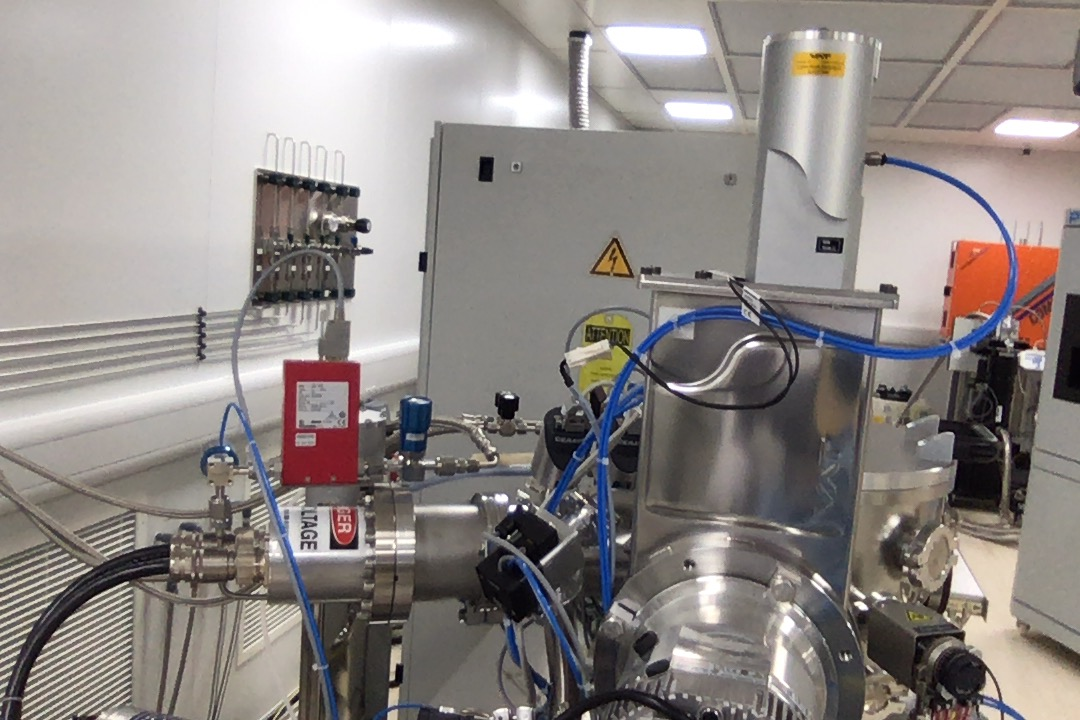
\includegraphics[height=7cm]{argon}
   \caption{\small     Argon      through     flow      meter     for
     etching\label{fig:argon}}
 \end{figure}


 \begin{enumerate}
 \item \cmd{Put the loadlock into \quote{process} mode button};
 \item \cmd{Enter the argon flow rate  in the very top box \quote{IBF
       Ar (20sscm)} \ira click the red traingles next to the argon}
 \end{enumerate}

 \subsubsection{Flushing controlled flow / static oxygen-argon line}
 \label{sec:flush-contr-flow}

\begin{framed}\noindent
  \textbf{Located on  the side  of plassys.  You  can admit  argon or
    oxygen either  through the red  flow meter or statically  via the
    needle valve}
\end{framed}

 \begin{figure}[h]
   \centering 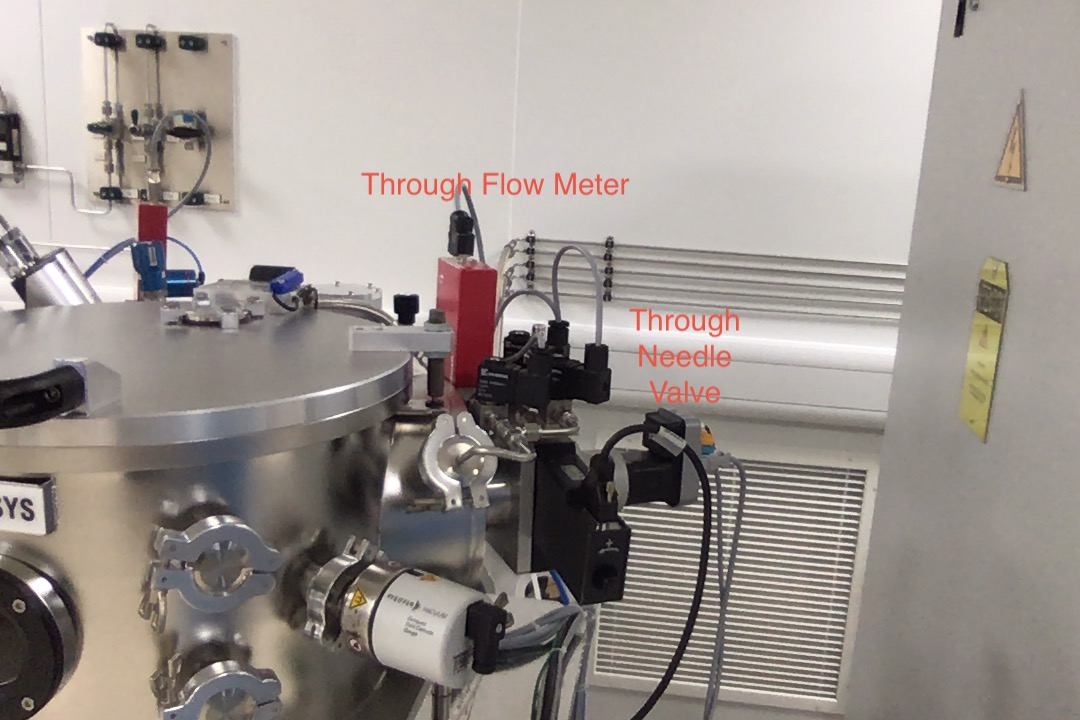
\includegraphics[height=7cm]{argon-oxygen}
   \caption{\small   Two   ways   to    admit   argon   and   oxygen:
     \textbf{statically}    and    \textbf{via     the    red    flow
       meter}\label{fig:argon-oxygen}}
 \end{figure}

 \begin{enumerate}
 \item Click ``static oxidation'' for the loadlock;
 \item Make sure valve you want to flush is open, \red{but never both
     the argon and oxygen!}
 \item Click triangle  next to needle valve on the  plassys menu (you
   may need to open the needle valve itself as well)
 \item \textbf{\red{Wait until 50mBar}} \ira pump again
 \end{enumerate}


 \begin{figure}[h]
   \centering \includegraphics[height=16cm]{argon-oxygen_plassys.png}
   \caption{\small     Controlling      of     oxygen-argon     flow.
     \textbf{Triangles} are for the computer.  \textbf{Yellow circles
       are                                                     manual
       taps.}\label{fig:argon-oxygen_plassys} \label{fig:argon-oxygen_plassys}}
 \end{figure}

 \newpage

%%% Local Variables:
%%% mode: latex
%%% TeX-master: "fat_manual"
%%% End:
